\section{Gestione dei dati Multimediali}
	
\clearpage

	
\subsection{ Recupero} 

L’aggiunta delle immagini richiede prima una fase di recupero. L’utente ha la possibilità di selezionare direttamente le immagini dal dispositivo utilizzato. In alternativa, sui dispositivi mobili, il sistema implementa una logica per rilevare automaticamente le foto scattate durante l’evento.

La possibilità di analizzare la galleria del dispositivo alla ricerca delle foto sussiste solo a seguito del permesso esplicito da parte dell’utente. Al primo accesso dell’applicazione verrà quindi richiesto il permesso all'accesso alla galleria, seguito dalla richiesta di poter creare notifiche. In caso tale concessione fosse negata, verrà richiesto ogni qual volta fosse reso necessario.

A seguito del termine di ogni evento, nel primo momento utile, l’applicativo esegue una ricerca delle foto scattate durante la sua intera durata. Nel caso in cui siano state rilevate immagini, vengono salvati i loro riferimenti in memoria locale, per poi notificare l’utente del loro ritrovamento. L’utente può quindi modificare la selezione, confermando o meno il caricamento delle foto trovate.



\begin{figure}[h!]
    \centering
    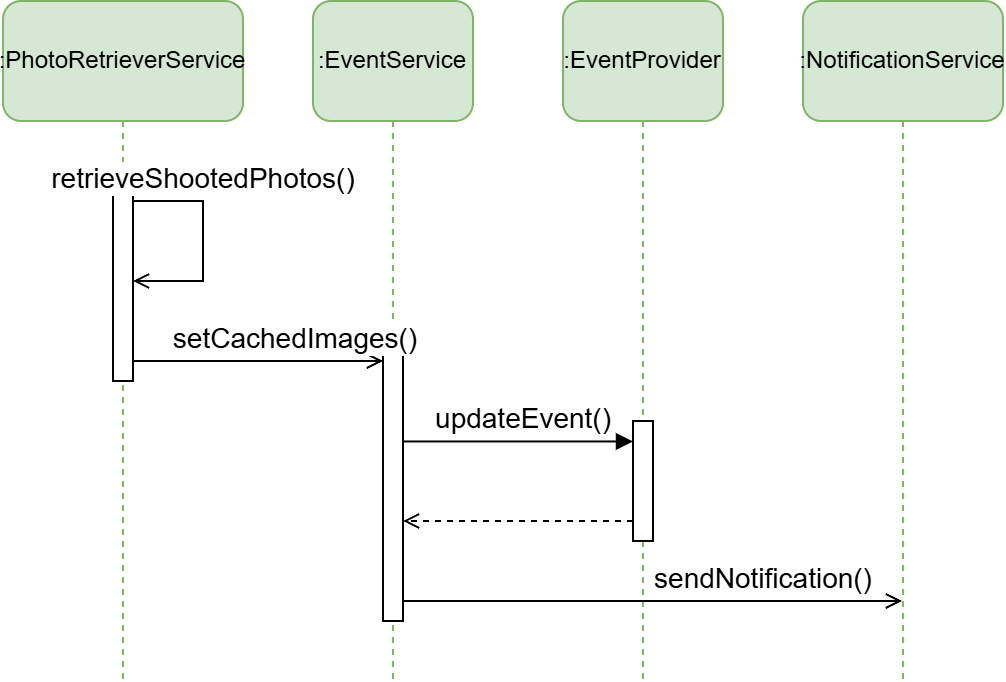
\includegraphics[width=\textwidth]{IIRecuperaImmagini.png}
    \caption{Interazione tra i componenti per il recupero delle immagini}
\end{figure}	





Pur risultando fondamentale per fornire un servizio trasparente con gli utenti, limitando disguidi e rischi dovuti ad un utilizzo inappropriato, la fase di conferma dell’utente presenta anche vantaggi prestazionali, mentre non costituisce un obbligo di natura legale. 

Le procedure di selezione e di recupero automatico delle immagini dalla galleria dell’utente sono contenute nelle modalità d’uso che l’utente deve accettare espressamente. Come previsto dalla normativa di tutela dell’immagine (C.C. art.10 e L. n.633/1941 artt. 96-97) e della privacy (GDPR: Reg.to UE 2016/679), la responsabilità per la pubblicazione delle immagini è in capo a chi realizza la foto, che ha l’obbligo di chiedere il consenso al/ai soggetti presenti nell’immagine. 


Come già affrontato nel capitolo precedente, richieste che prevedono la modifica di uno stesso componente comportano vincoli di concorrenza per l’accesso alla risorsa interessata. Il termine di un evento condiviso con più utenti crea il rischio  della ricezione contemporanea di più richieste di aggiunta di immagini convergenti sullo stesso elemento. L’attesa della selezione introduce un ritardo tra la fine dell’evento e il caricamento delle immagini interessate. La differita comporta una diffusione delle richieste maggiore nel tempo, riducendo l’eventualità di collisione di due richieste sullo stesso evento.

Al termine della selezione, le immagini verranno inviate al server, per essere salvate e allegate all’evento. 


\subsection{ Salvataggio}

A differenza dei dati normalmente scambiati, i file multimediali presentano dimensioni significativamente superiori, con differenze che si manifestano su ordini di grandezza rilevanti. 

Un salvataggio allineato ai dati degli elementi logici comporterebbe un rallentamento di tutte le operazioni, con impatto significativo sulle prestazioni del sistema. Si necessita quindi una gestione della memoria creata appositamente. 
Le dimensioni delle immagini e dei video influenzano inoltre il tempo di elaborazione e il volume delle richieste, richiedendo risorse maggiori a tutti i componenti del sistema. Infine, vista la possibilità di allegare più file ad un evento, il tempo maggiore di caricamento delle immagini potrebbe portare a tempi lunghi di transazioni per le modifiche degli eventi.


\subsubsection{Persistenza}

La visualizzazione dei file multimediali ricopre una priorità minore rispetto alle altre funzionalità offerte dall’applicazione. Si può quindi accettare un maggior tempo di caricamento se questo comporta una riduzione della latenza delle altre operazioni. Il salvataggio dei file multimediali sul database centrale aumenterebbe significativamente il volume specifico delle richieste, comportando un maggiore impiego di risorse computazionali e un aumento dei tempi di caricamento. Tale fenomeno potrebbe incidere negativamente sulle prestazioni complessive del sistema, penalizzando l'esecuzione simultanea di altre operazioni.

Attraverso la separazione dell'oggetto logico dal suo valore binario, si può distinguere la relazione tra il file e l'evento dai dati binari che lo compongono. Una volta recuperati i riferimenti ai file multimediali associati all’evento, sarà quindi possibile ottenere i loro valori binari in un secondo momento. Il modello del dominio visto in precedenza mostra la relazione logica tra l’evento e i file associati(Photo).
Data necessità e la possibilità di salvare i dati dei file multimediali su risorse differenti rispetto al database centrale, occorre individuare la soluzione più adatta per la loro persistenza.

Le principali tipologie di servizi in cloud per il salvataggio dei file multimediali si suddividono in Object, File e Block Storage.

Gli Object Storage gestiscono i file su un unico livello, con la possibilità di aggiungere metadati agli oggetti.  Ad ogni elemento viene associato un codice univoco attraverso il quale sarà possibile recuperarlo. L’accesso ai dati avviene generalmente tramite API RESTful, che oltre a dare la possibilità di gestire permessi, permette l’utilizzo su ampia scala. L’unico livello di indirizzamento permette una scalabilità illimitata, e il prezzo varia solo in base alla quantità dei dati salvati. 

I File Storage organizzano i file in una struttura gerarchica di cartelle e sottocartelle, che consente una maggiore facilità di accesso e gestione dei file. La particolarità della struttura permette un controllo ulteriore dei permessi degli utenti, inoltre fornisce la compatibilità con protocolli di accesso basati sui file systems, permettendone l’integrazione con tecnologie particolari. La scalabilità di questa tecnologia dipende molto dall’organizzazione dei file, e dalla loro quantità. La sua capacità dipende dal piano selezionato, così come il prezzo.


I Block Storage gestiscono la memoria tramite blocchi logici di dati, salvati separatamente con identificatori univoci. I blocchi vengono associati a volumi che ne permettono l’interazione, fornendo la possibilità di variare la tipologia di interazione con i blocchi. Permettono ampie prestazioni di recupero e modifica dei dati ma le prestazioni variano in base alla quantità di dati presenti. La scalabilità è limitata alla capacità assegnata al volume. Il prezzo è elevato, soprattutto per grandi moli. 

La tecnologia più adatta al salvataggio dei file multimediali del progetto è di tipo Object Storage. Assicurando una scalabilità infinita, risponde alla necessità di salvare grandi quantità di elementi con una scarsa relazione tra loro. L’identificazione univoca permette un'alta velocità di ritrovamento dei dati, così come la risposta prestazionale a numerose richieste contemporanee.

Il servizio di Object Storage fornito da Azure è Azure Blob Storage (ABS). ABS prevede un'organizzazione centrata su entità logiche Container che raggruppano più file multimediali, introducendo un livello di indirizzamento aggiuntivo. Permette l’accesso in lettura tramite protocollo API RESTFul, e l’aggiunta di elementi tramite autenticazione. Per ogni evento si crea un Container associato, che conterrà le immagini relative.

Terminata la selezione delle immagini, prima dell’invio delle immagini al server, i dispositivi comprimono i file. Questo permette di ridurre la banda consumata e la quantità di dati totale scambiata, risparmiando ulteriore carico computazionale al server.


Il server, ricevuta la richiesta, ha quindi il compito di eseguire un controllo sui permessi necessari, per poi caricare le immagini sul Container dell’evento. Al seguito del termine del caricamento, aggiorna l’evento sul database con i riferimenti alle immagini aggiunte. Infine, notifica gli utenti della modifica avvenuta.
La visualizzazione di un evento con immagini allegate comporta la richiesta parallela delle singole immagini dal dispositivo ad ABS. Le immagini saranno identificate univocamente dall'associazione dell’hash dell’immagine con l’hash del container associato all’evento.


\begin{figure}[h!]
    \centering
    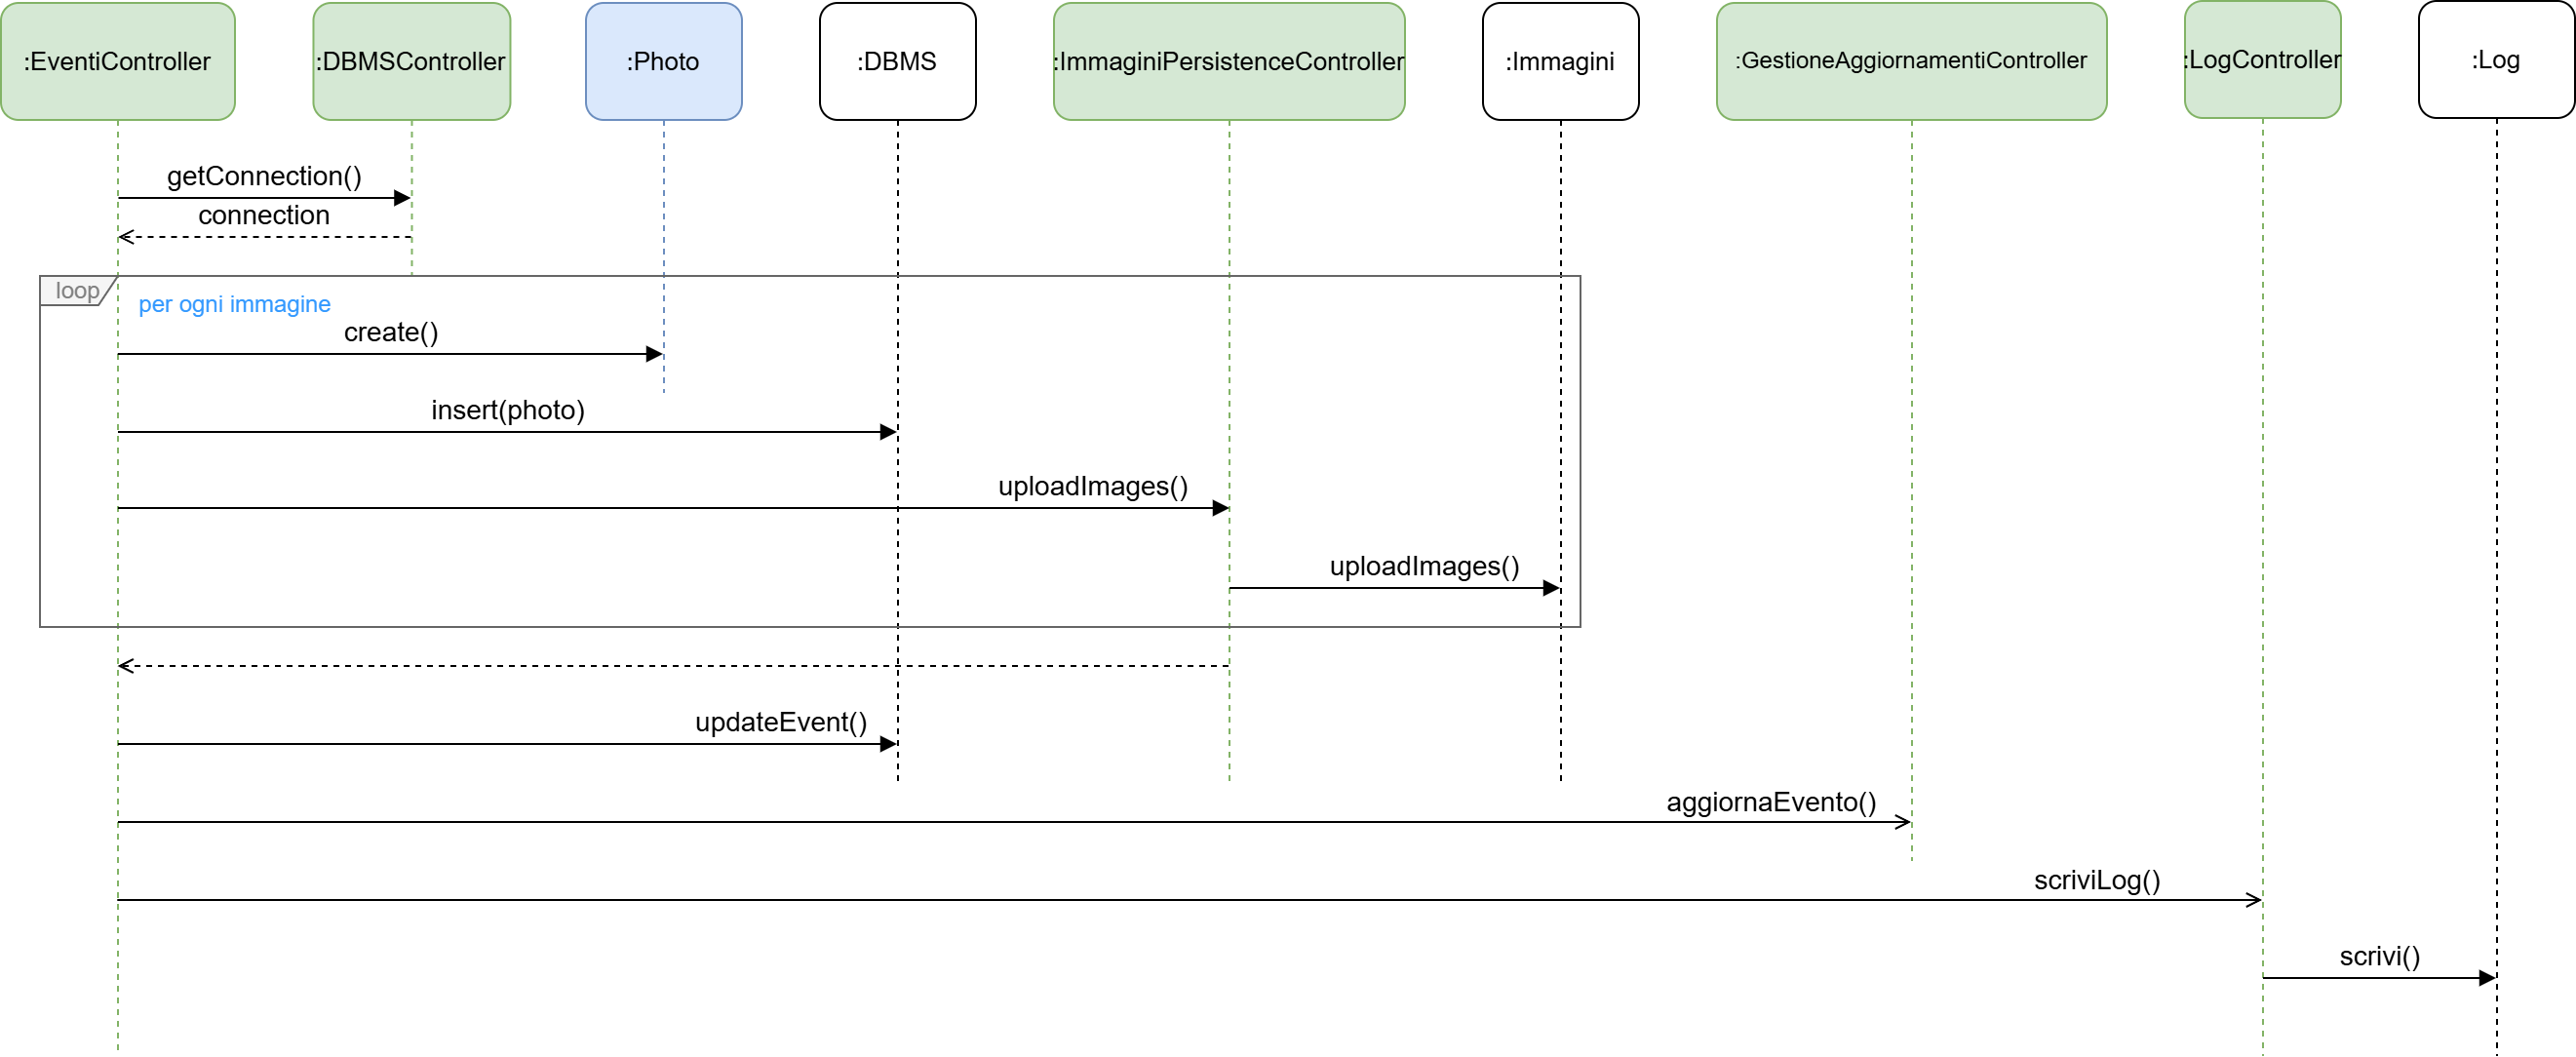
\includegraphics[width=\textwidth]{PIConfermaImmagini2.png}
    \caption{Interazione progettuale del server per il caricamento delle immagini }
\end{figure}	

L’accesso in lettura alle immagini però risulta così pubblico: la mancata definizione di ruoli comporta la carenza di controlli sull’autorizzazione delle richieste. Il problema si considera però ampiamente mitigato grazie alla creazione di hash randomici sufficientemente lunghi a rendere minima la probabilità di collisione.  La fruizione alle immagini senza la conoscenza degli hash, che richiede numerosi tentativi casuali nella speranza di trovare una combinazione corretta, risulta così molto improbabile e, nel caso di un attacco andato a buon fine, non fornisce ulteriori informazioni sul resto delle immagini.



\clearpage

\subsubsection{ Concorrenza }

Il caricamento delle immagini dalle Azure Functions al Container relativo all’evento è un’operazione lunga, soprattutto rispetto a tutte le altre eventualità. Il collegamento del server con il database relazionale comporta scelte di dominio e di sviluppo volte a permettere un uso ottimale delle sue connessioni, per ridurre al minimo il tempo di blocco delle risorse.

Per poter inviare i dati è necessario essere a conoscenza dell’hash dell’elemento Photo che andrà a corrispondere al file. L’hash viene generato nel momento della creazione dell’oggetto. Il suo salvataggio in memoria è bene che avvenga però solo a seguito dell’avvenuto caricamento del file multimediale, per evitare inutili scritture e cancellazioni sul database. Il momento della creazione di Photo è necessario che sia perciò distinto dal momento del suo salvataggio.

EF Core, per realizzare un’astrazione ad alto livello della relazione con il database, fornisce una rappresentazione logica degli elementi, mantenendo un collegamento con il loro corrispettivo fisico. Permette quindi di creare un oggetto subito e di  memorizzarlo in un secondo momento. 

La relazione uno a molti tra gli eventi e le immagini viene mappata fisicamente sugli oggetti Photo, salvando l’identificativo dell’Event associato. Nel momento del salvataggio verrà così modificata solo la tabella relativa a Photo. Tuttavia, il momento del suo salvataggio richiede il blocco in scrittura anche dell’Event interessato. L’oggetto Event risulta infatti coinvolto da un punto di vista logico, come si evince anche dalla presenza tra i suoi attributi virtuali(ovvero descritti dall’incrocio di dati da altre fonti) della lista delle immagini.

La parallelizzazione della trasmissione dei file multimediali al Container permette la minimizzazione del tempo necessario per lo svolgimento della richiesta. L’aggiunta dell’oggetto Photo al termine di ogni caricamento porterebbe al rischio di conflitti sullo stesso Event e il sovraccarico del database. Verranno quindi conservati temporaneamente gli oggetti logici Photo delle trasmissioni avvenute con successo, per salvarli poi in un’unico momento.

L’inserimento di tutti gli elementi Photo validi nella stessa transazione comporta  l'ottimizzazione dell’impatto sul database, riducendo i tempi di blocco sull’Event e quindi minimizzando le possibilità di collisione tra le richieste coinvolte.

\begin{figure}[h!]
    \centering
    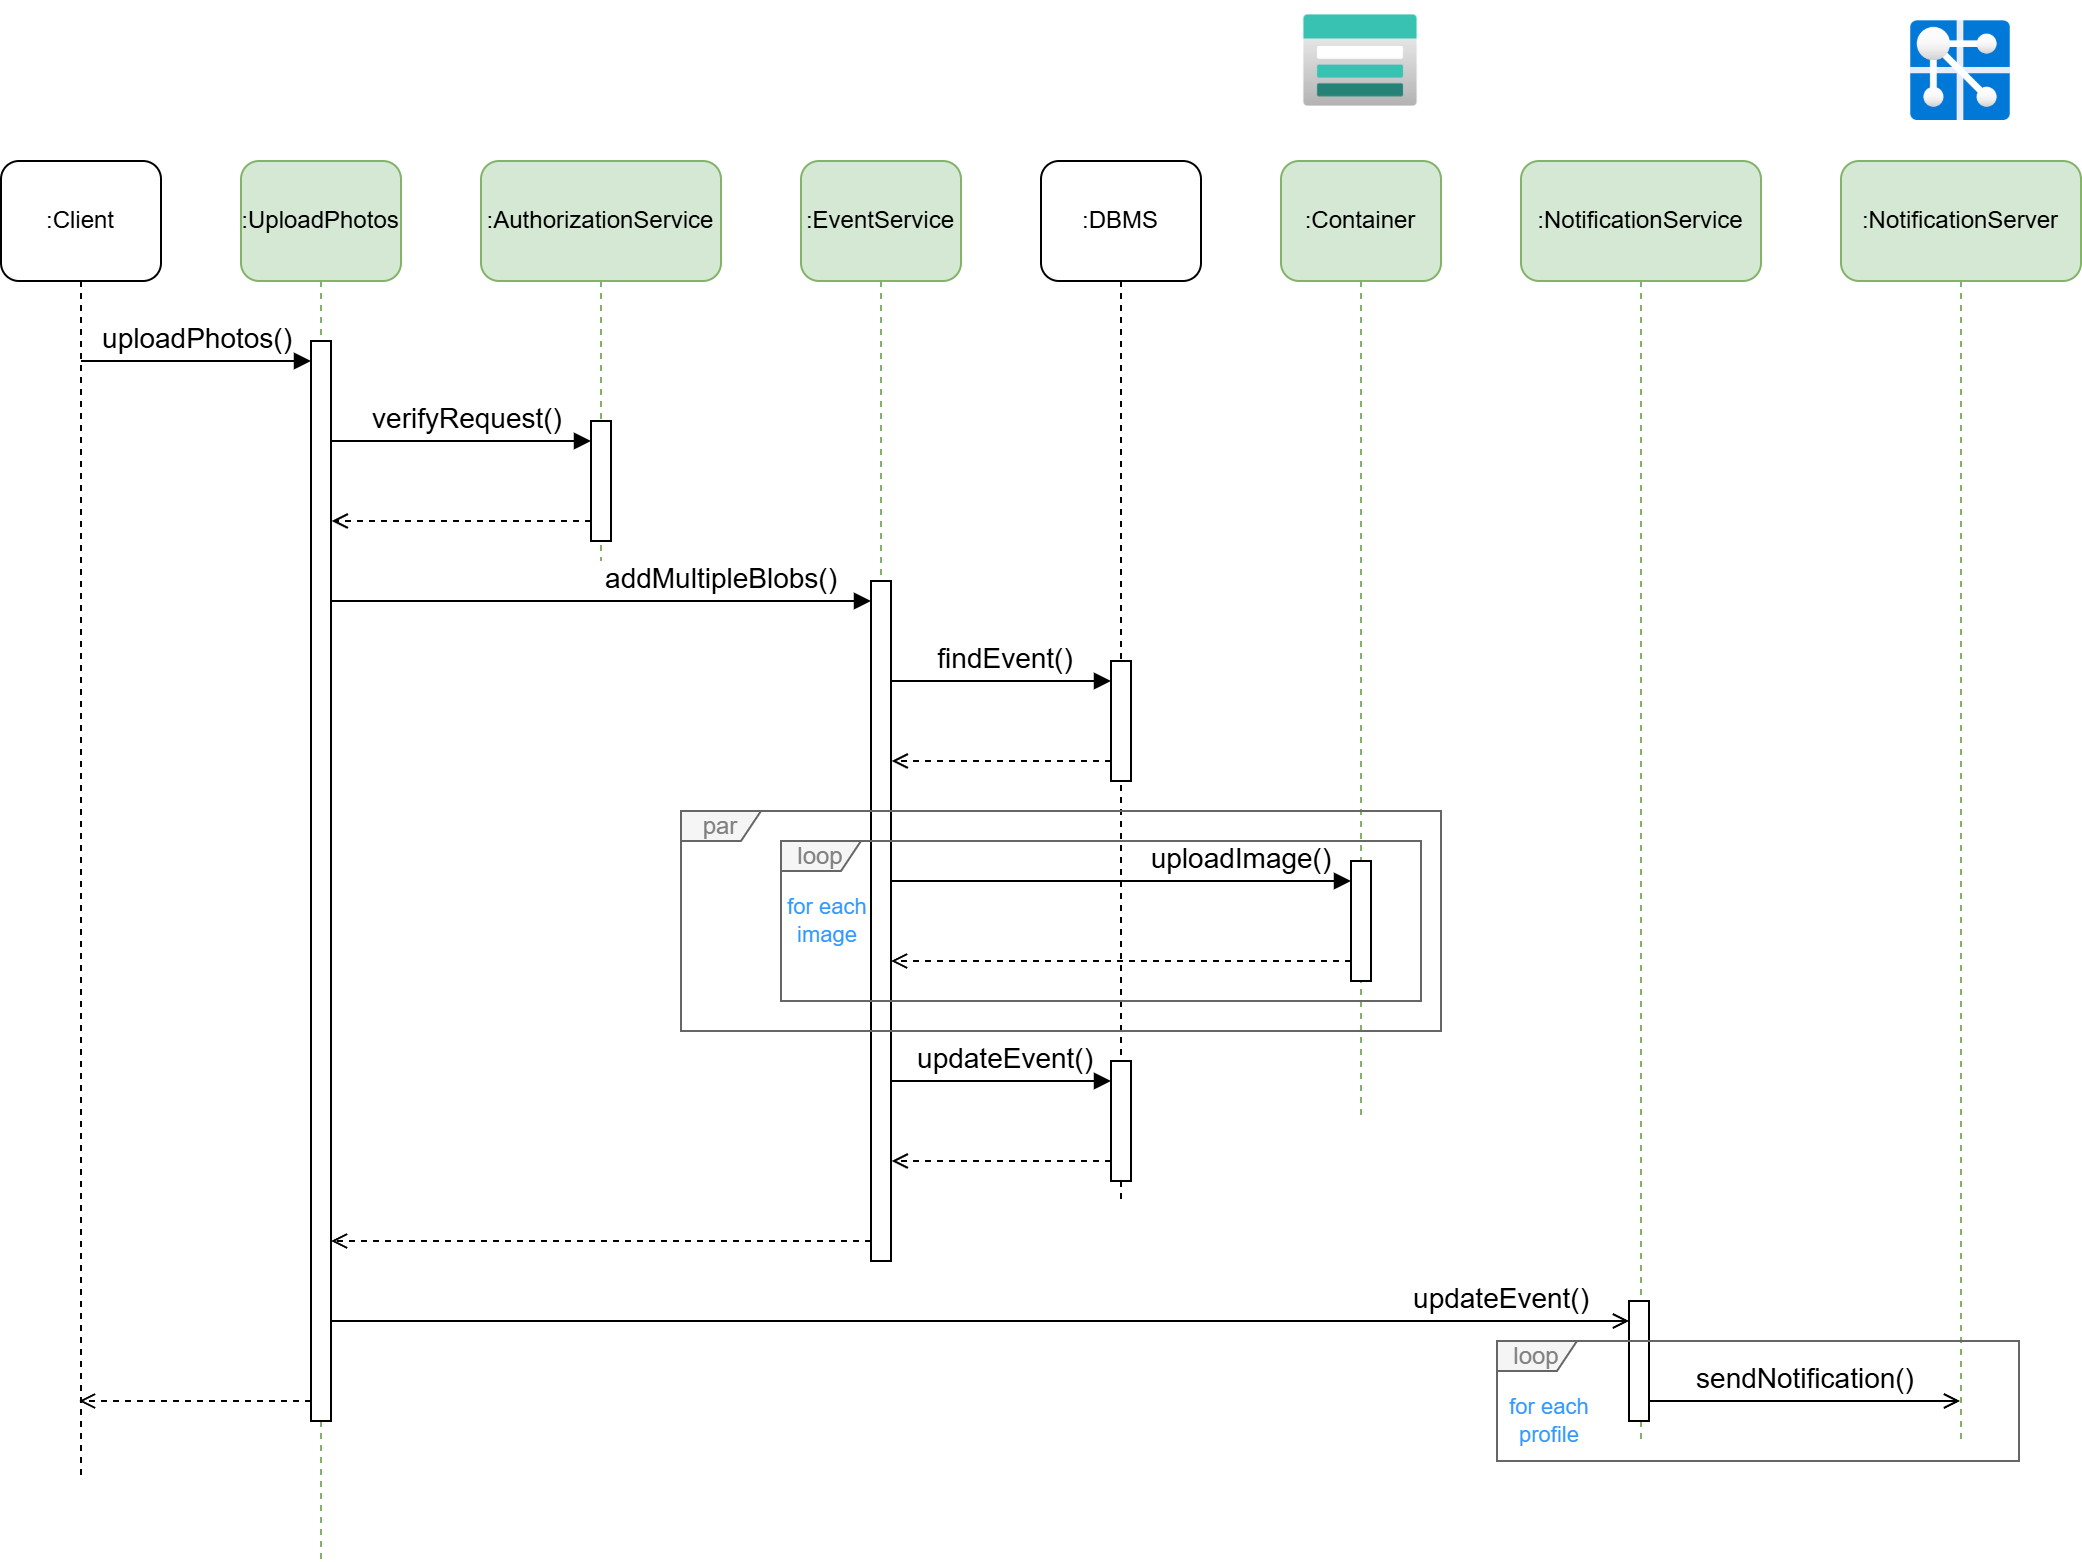
\includegraphics[width=\textwidth]{IICaricaImmagini.png}
    \caption{Interazione logica del server per il caricamento delle immagini }
\end{figure}

\clearpage